% Copyright 2026 Sreeram Anil
% SPDX-License-Identifier: CC-BY-4.0
% =============================================================================
%  Innovation-based adaptive estimation (windowed covariance matching)
% =============================================================================
\chapter{Innovation-based adaptive estimation (IAE-AKF)}
\label{ch:iaeakf}

\section*{At a glance}
\begin{tabular}{@{}l>{\raggedright\arraybackslash}p{0.76\textwidth}@{}}
Family & Adaptive Kalman \\
Header & \texttt{include/estkit/filters/iae\_akf.hpp} \\
Registered name & \texttt{IAE-AKF} \\
State dimension & $n_x = 4$ (cell model) --- generic in $n_x, n_u, n_y$; window $N$ is a template parameter \\
Cost per step & EKF $+\,\mathcal{O}(n_y^2)$; $\approx 500$\,ns/step measured; $N n_y$ reals of buffer, no heap \\
Primary references & \cite{mehra1970,mohamed1999adaptive,maybeck1979,jazwinski1970} \\
\end{tabular}

\section{Motivation and aerospace/BMS relevance}
Mehra's 1970 paper \cite{mehra1970} is the origin of the whole family of adaptive Kalman filters
that work by \emph{covariance matching}.  The observation is elementary and powerful: a Kalman
filter publishes, at every step, a prediction of the second-order statistics of its own innovation
sequence, $\mS_k = \mH_k\Pminus_k\mH_k^\T + \mR_k$.  If the filter's noise model is right, the
empirical covariance of the innovations must match $\mS_k$; if it does not, the mismatch tells us
by how much, and in which direction, the model is wrong.  Mehra showed that for a linear
time-invariant system the full autocorrelation function of the innovations identifies both $\mQ$
and $\mR$ (up to the well-known identifiability restrictions), and that the zero-lag term alone
identifies $\mR$ directly.

Mohamed and Schwarz \cite{mohamed1999adaptive} turned this into the standard practical recipe used
throughout navigation: estimate the innovation covariance over a \emph{moving window} of the last
$N$ samples and subtract the part the filter attributes to state uncertainty.  Their paper calls
the resulting estimator IAE (innovation-based adaptive estimation), distinguishing it from RAE
(residual-based adaptive estimation), which uses the a-posteriori residual instead.  IAE became the
workhorse of loosely coupled INS/GPS integration, where the GPS pseudo-range noise varies by an
order of magnitude between open sky and urban canyon; the battery analogue is a cell-voltage
channel whose effective noise changes with the switching state of the traction inverter, or a
voltage multiplexer that intermittently returns a stale sample.

Compared with the Sage--Husa recursion of \cref{ch:sagehusaakf}, the windowed estimator has a
sharper time--variance trade-off: a rectangular window of length $N$ forgets completely after $N$
samples instead of exponentially, so the response to a step change in the noise level is a ramp of
exactly $N$ samples rather than an exponential tail.  It costs $N n_y$ reals of ring buffer.

\section{Problem statement and assumptions}
The plant is \eqref{eq:sh:proc}--\eqref{eq:sh:meas} of \cref{ch:sagehusaakf}.  Define the
a-priori innovation
\begin{equation}
\bm{e}_k \triangleq \vy_k - h(\xminus_k,\vu_k) \in \real^{n_y},
\label{eq:iae:innov}
\end{equation}
where $\xminus_k$ is the one-step prediction of the state.  We seek $\hat{\mR}_k$ under

\begin{assumption}\label{as:iae:white}
The filter is close enough to consistency that $\bm{e}_k$ is approximately zero-mean and white; then
$\E{\bm{e}_k\bm{e}_k^\T} = \mH_k\Pminus_k\mH_k^\T + \mR_k$.
\end{assumption}
\begin{assumption}\label{as:iae:stat}
$\mR_k$ and $\mH_k\Pminus_k\mH_k^\T$ are approximately constant over the window
$\{k-N+1,\dots,k\}$.
\end{assumption}

\section{Derivation}

\subsection{Innovation covariance and the matching condition}
For the linearised filter, propagate the estimation error $\tilde{\vx}^-_k = \vx_k - \xminus_k$:
\begin{equation}
\bm{e}_k = \vy_k - h(\xminus_k,\vu_k) = \mH_k\tilde{\vx}^-_k + \vv_k + \mathcal{O}(\|\tilde{\vx}^-_k\|^2).
\label{eq:iae:elin}
\end{equation}
$\vv_k$ is independent of $\tilde{\vx}^-_k$ (which depends only on data up to $k-1$ and on
$\vw_{0:k-1}$), so
\begin{equation}
\mC_{v,k} \triangleq \E{\bm{e}_k\bm{e}_k^\T} = \mH_k\,\E{\tilde{\vx}^-_k\tilde{\vx}^{-\T}_k}\,\mH_k^\T + \mR_k
= \mH_k\Pminus_k\mH_k^\T + \mR_k ,
\label{eq:iae:match}
\end{equation}
provided the filter's $\Pminus_k$ equals the true prediction-error covariance.  Equation
\eqref{eq:iae:match} is the \emph{covariance-matching condition}.  Solving it for $\mR_k$,
\begin{equation}
\boxed{\;\hat{\mR}_k = \hat{\mC}_{v,k} - \mH_k\Pminus_k\mH_k^\T\;}
\label{eq:iae:R}
\end{equation}
with the sample estimate over the moving window
\begin{equation}
\hat{\mC}_{v,k} = \frac{1}{N}\sum_{j=k-N+1}^{k} \bm{e}_j\bm{e}_j^\T .
\label{eq:iae:Cv}
\end{equation}
This is Mohamed and Schwarz's IAE \cite[Eq.~(16)]{mohamed1999adaptive}; Mehra
\cite[Sec.~III]{mehra1970} derives the same expression as the zero-lag element of the innovation
autocorrelation sequence.

\subsection{Statistical properties}
Under \cref{as:iae:white} and \cref{as:iae:stat} the estimator \eqref{eq:iae:R} is unbiased:
$\E{\hat{\mR}_k} = \mC_{v,k} - \mH_k\Pminus_k\mH_k^\T = \mR_k$.  Its variance follows from the
Wishart distribution of \eqref{eq:iae:Cv}: for $n_y=1$,
\begin{equation}
\frac{\Var{\hat{R}_k}}{\big(\mH_k\Pminus_k\mH_k^\T+R_k\big)^2} = \frac{2}{N},
\label{eq:iae:var}
\end{equation}
i.e.\ a relative standard deviation of $\sqrt{2/N}$ on the \emph{innovation} variance, which is
inflated by the factor $(1 + \mH\Pminus\mH^\T/R)^2$ when referred to $\hat R$ itself.  With $N=80$
the relative error is $16\,\%$; the response time to a step change in the noise level is exactly
$N$ samples.  Choosing $N$ is therefore the same bias--variance compromise as choosing $b$ in
Sage--Husa, with $N \leftrightarrow 2/(1-b)$ giving comparable variance.

\subsection{Positive definiteness}
The difference in \eqref{eq:iae:R} is not guaranteed positive definite: when the true $\mR$ is small
compared with the state-uncertainty contribution, or when the window happens to contain unusually
small innovations, $\hat{\mR}_k$ can have non-positive diagonal entries.  The standard remedy, and
the one implemented here, is a projection onto a bounded positive-definite set,
\begin{equation}
\hat R_{k,ii} \gets \mathrm{clamp}\!\left(\hat R_{k,ii},\; \rho_{\min} R_{ii},\; \rho_{\max} R_{ii}\right),
\qquad
|\hat R_{k,ij}| \le 0.99\sqrt{\hat R_{k,ii}\hat R_{k,jj}},
\label{eq:iae:floor}
\end{equation}
where $R_{ii}$ is the nominal model value.  The second condition enforces the Cauchy--Schwarz bound
on the off-diagonal entries, which for $n_y\le 2$ is sufficient for positive definiteness and for
larger $n_y$ is a cheap necessary condition.  For the cell model $n_y=1$ and only the clamp acts.

\subsection{Why the process-noise covariance is not adapted}
The companion IAE estimator for the process noise,
$\hat{\mQ}_k = \hat{\mC}_{\Delta x,k} + \Pplus_k - \mF_{k-1}\Pplus_{k-1}\mF_{k-1}^\T$ with
$\hat{\mC}_{\Delta x,k}$ the windowed covariance of the state correction $\mK_j\bm{e}_j$
\cite[Eq.~(17)]{mohamed1999adaptive}, requires $N \gg n_x^2$ samples to be usable and, like the
Sage--Husa version, suffers from the fundamental non-identifiability of $(\mQ,\mR)$ from a single
output record \cite{mehra1970}: only $n_y(n_y+1)/2 \cdot n_x$ elements of the autocorrelation
sequence are informative, which is generally fewer than the $n_x(n_x+1)/2$ unknowns in $\mQ$.  For
the ECM, $\mQ$ is moreover structured (it is the image of the current-sensor noise through
$\partial f/\partial i$ plus a diagonal floor), so an unstructured estimate would discard known
information.  $\mQ$ adaptation is therefore not offered.

\section{Algorithm}
\begin{algorithm}[H]
\caption{IAE-AKF --- one sampling period}
\begin{algorithmic}[1]
\Require $\xplus_{k-1},\Pplus_{k-1},\vu_{k-1},\vy_k,\vu_k$, ring buffer $\{\bm{e}_{k-N},\dots,\bm{e}_{k-1}\}$, running sum $\Sigma$
\State \textbf{Time update:} $\xminus_k\gets f(\xplus_{k-1},\vu_{k-1})$;\quad
       $\Pminus_k\gets\mF\Pplus_{k-1}\mF^\T+\mQ_k$
\State \textbf{Innovation:} $\mH\gets\partial h/\partial\vx|_{\xminus_k}$;\quad $\bm{e}_k\gets\vy_k-h(\xminus_k,\vu_k)$
\State \textbf{Ring buffer:} if full, $\Sigma\gets\Sigma-\bm{e}_{k-N}\bm{e}_{k-N}^\T$;\quad
       store $\bm{e}_k$;\quad $\Sigma\gets\Sigma+\bm{e}_k\bm{e}_k^\T$
\State \textbf{Covariance matching} (if buffer has $\ge N_{\min}$ entries):
       $\hat{\mC}_v\gets\Sigma/n$;\quad $\hat{\mR}_k\gets\hat{\mC}_v-\mH\Pminus_k\mH^\T$;\quad apply \eqref{eq:iae:floor}
\State \textbf{Gain:} $\mS_k\gets\mH\Pminus_k\mH^\T+\hat{\mR}_k$;\quad $\mK_k\gets\Pminus_k\mH^\T\mS_k\inv$
\State \textbf{State update:} $\xplus_k\gets\xminus_k+\mK_k\bm{e}_k$
\State \textbf{Covariance (Joseph):} $\Pplus_k\gets(\mI-\mK_k\mH)\Pminus_k(\mI-\mK_k\mH)^\T+\mK_k\hat{\mR}_k\mK_k^\T$
\State \textbf{Constrain:} $\xplus_k\gets\mathrm{constrain}(\xplus_k)$
\Ensure $\xplus_k,\Pplus_k,\hat{\mR}_k$
\end{algorithmic}
\end{algorithm}
The running sum $\Sigma$ makes the window update $\mathcal{O}(n_y^2)$ instead of
$\mathcal{O}(N n_y^2)$; the buffer is a fixed-size array, so no heap is used.  Note that
$\hat{\mR}_k$ is computed \emph{before} the gain, so the current sample already benefits from the
adaptation --- unlike the Sage--Husa recursion, which necessarily updates $\hat{\mR}$ after the
state update because it uses the a-posteriori residual.

\section{Application to the battery model}
With $n_y=1$ the estimator reduces to
$\hat R_k = \frac{1}{N}\sum_j e_j^2 - \big(\partial\ocv/\partial\soc\big)^2 P^-_{\soc\soc}
- \dots$, i.e.\ a plain running mean of squared voltage innovations, less the (usually tiny)
model-uncertainty contribution.  The window is a template parameter, \texttt{IaeAkf<Model, NWIN>};
the registered estimator uses $N = 80$ samples $=\SI{8}{\second}$.  The choice sits in the middle
of the $N=50$--$100$ range used in the navigation literature and was checked against $N\in\{50,100\}$:
the steady-state metrics vary by less than $20\,\%$ and the ranking against the EKF does not change.
At \SI{10}{\hertz}, $N=80$ gives a $16\,\%$ relative accuracy on the variance estimate and an
\SI{8}{\second} reaction time, which is short compared with the slow RC time constant
$\tau_2=\SI{120}{\second}$ of the cell and long compared with the fast one, $\tau_1=\SI{5}{\second}$.
The bounds are $\rho_{\min}=0.05$, $\rho_{\max}=5\times10^3$, i.e.\
$\hat\sigma_v\in[0.47,148]\,\si{\milli\volt}$; adaptation starts only once the window is full
(\texttt{min\_samples} $=N$), so the initial transient of the filter does not enter the estimate.
An optional first-order smoother on $\hat{\mR}$ (\texttt{opts.smooth}) is provided but defaults to
off.

\section{Implementation notes}
\begin{itemize}[leftmargin=1.4em]
\item \textbf{Buffer.}  \texttt{Y buf\_[NWIN]} plus one $n_y\times n_y$ running sum; for the cell
      model that is $80$ doubles $=640$\,bytes.  Wrapping is done with a single modulo on the
      head index.  Deleting the oldest outer product and adding the newest keeps the cost at
      $\mathcal{O}(n_y^2)$ per sample.
\item \textbf{Drift.}  Maintaining $\Sigma$ incrementally accumulates round-off over long runs.  For
      $n=2\times10^4$ samples in double precision this is far below the $16\,\%$ statistical error;
      in the float32 build it was verified to leave the metrics unchanged to three digits.  If a
      run of $10^7$ samples were required, periodic re-summation of the buffer would be the fix.
\item \textbf{Ordering.}  $\hat{\mR}_k$ uses $\Pminus_k$ \emph{before} the update, which is the
      quantity that appears in \eqref{eq:iae:match}.  Using $\Pplus_k$ here is a common
      implementation error and biases $\hat{\mR}$ upwards.
\item \textbf{Cold start.}  Before the window is full the filter runs with the nominal model $\mR$;
      this avoids the very noisy one- or two-sample variance estimates that a naive implementation
      would produce.
\item \textbf{Cost.}  Measured \SI{500}{\nano\second}/step against the EKF's
      \SI{478}{\nano\second}/step (a $5\,\%$ overhead).  It is the cheapest of the adaptive filters in
      this family because it needs no extra evaluation of $h$.  On a \SI{400}{\mega\hertz} Cortex-M7
      this scales to roughly \SI{6}{\micro\second}/step.
\item \textbf{Limitations.}  \cref{as:iae:white} is violated whenever the innovations are coloured,
      which happens with slow un-modelled dynamics (cold cell, hysteresis mismatch); the estimator
      then over-estimates $\mR$.  The rectangular window also means a single very large innovation
      stays in the estimate at full weight for exactly $N$ samples and then disappears abruptly,
      which produces a small step in the gain.
\end{itemize}

\section{Benchmark results}
% Copyright 2026 Sreeram Anil
% SPDX-License-Identifier: CC-BY-4.0
\begin{table}[H]\centering\footnotesize\setlength{\tabcolsep}{4pt}
\caption{IAE-AKF: cell-level benchmark on the eVTOL mission (mean over seeds; RMSE and max error in \% SOC; $t_\mathrm{conv}$: first time the error stays below 2\,\% for 60\,s, -- = never; EKF reference: steady-state RMSE of the plain EKF on the same data).}\label{tab:cell_IAEAKF}
\begin{tabular}{llrrrrrcrr}\toprule
plant & scenario & RMSE & RMSE$_\mathrm{ss}$ & max & $t_\mathrm{conv}$ [s] & RMSE$_v$ [mV] & div. & EKF ref. & ns/step \\ \midrule
ECM & nominal & 0.22 & 0.04 & 1.08 & 0 & 0.79 & no & 0.05 & 500 \\
ECM & init\_error & 0.12 & 0.07 & 0.60 & 0 & 2.12 & no & 0.05 & 499 \\
ECM & current\_bias & 0.53 & 0.62 & 1.39 & 0 & 0.87 & no & 0.61 & 499 \\
ECM & noise\_step & 0.22 & 0.04 & 1.08 & 0 & 1.01 & no & 0.12 & 499 \\
ECM & outliers & 0.41 & 0.11 & 2.92 & 2 & 1.04 & no & 0.21 & 501 \\
ECM & cold & 0.19 & 0.16 & 1.17 & 0 & 1.89 & no & 0.16 & 498 \\
ECM & hot & 0.19 & 0.03 & 1.01 & 0 & 0.54 & no & 0.03 & 499 \\
ECM & aged\_cell & 1.06 & 1.21 & 2.61 & 0 & 24.50 & no & 1.52 & 500 \\
ECM & param\_mismatch & 0.85 & 1.01 & 1.69 & 0 & 7.54 & no & 1.36 & 499 \\
ECM & sensor\_dropout & 0.20 & 0.05 & 1.08 & 0 & 0.90 & no & 0.46 & 498 \\
ECM & preisach & 0.61 & 0.20 & 1.82 & 0 & 0.81 & no & 0.20 & 500 \\
ECM & combined & 4.89 & 2.01 & 11.44 & 1448 & 16.50 & no & 12.44 & 501 \\
\midrule
SPM & nominal & 2.94 & 3.02 & 3.54 & 0 & 1.43 & no & 3.73 & 471 \\
SPM & init\_error & 3.56 & 3.56 & 4.49 & 9 & 2.42 & no & 3.81 & 469 \\
SPM & current\_bias & 4.76 & 5.45 & 6.10 & 0 & 1.71 & no & 5.69 & 470 \\
SPM & noise\_step & 2.94 & 3.02 & 3.54 & 0 & 2.30 & no & 3.30 & 473 \\
SPM & outliers & 2.58 & 2.58 & 3.91 & 0 & 2.30 & no & 1.99 & 475 \\
SPM & cold & 2.70 & 2.54 & 3.58 & 0 & 18.15 & no & 7.35 & 466 \\
SPM & hot & 2.13 & 2.19 & 2.53 & 0 & 0.75 & no & 2.16 & 472 \\
SPM & param\_mismatch & 1.14 & 1.20 & 2.00 & 0 & 4.47 & no & 3.13 & 469 \\
SPM & sensor\_dropout & 3.12 & 3.19 & 3.79 & 0 & 2.09 & no & 5.31 & 472 \\
\bottomrule\end{tabular}\end{table}

\begin{figure}[H]\centering
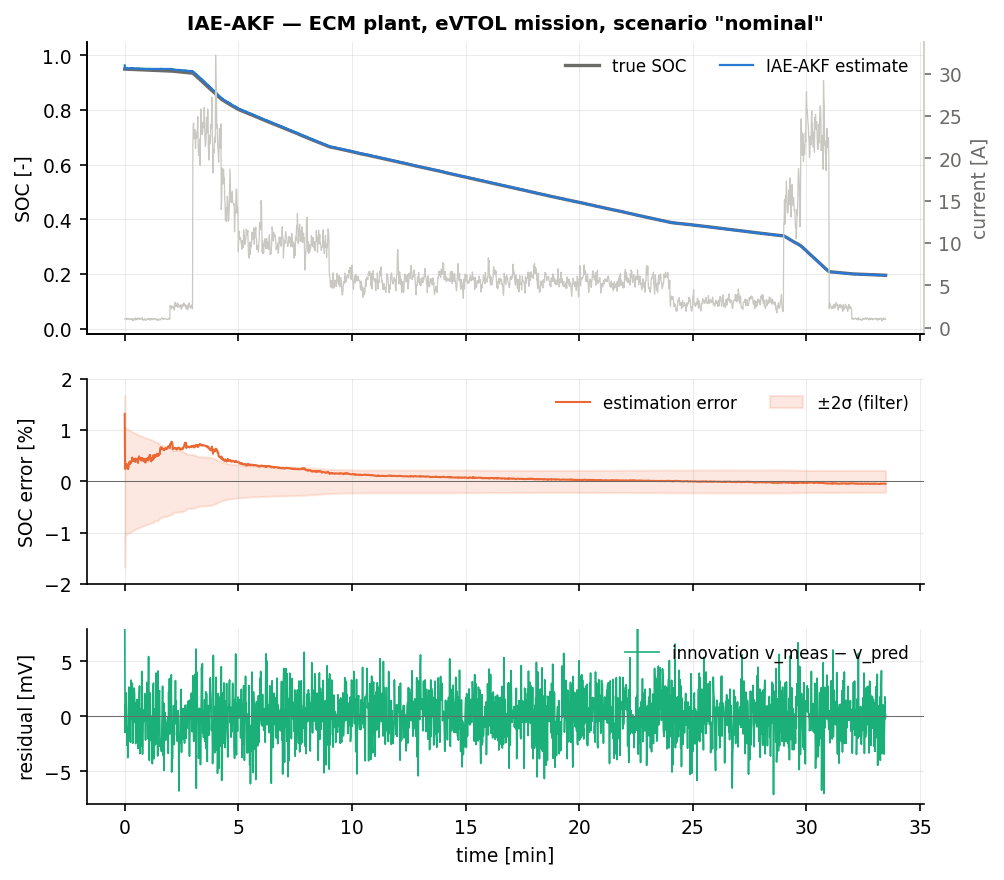
\includegraphics[width=\textwidth]{figures/cell_IAEAKF_nominal.png}
\caption{IAE-AKF on the nominal eVTOL mission: true and estimated SOC (top), estimation error with the $\pm 2\sigma$ band when available (middle), voltage residual (bottom).}
\end{figure}
\begin{figure}[H]\centering
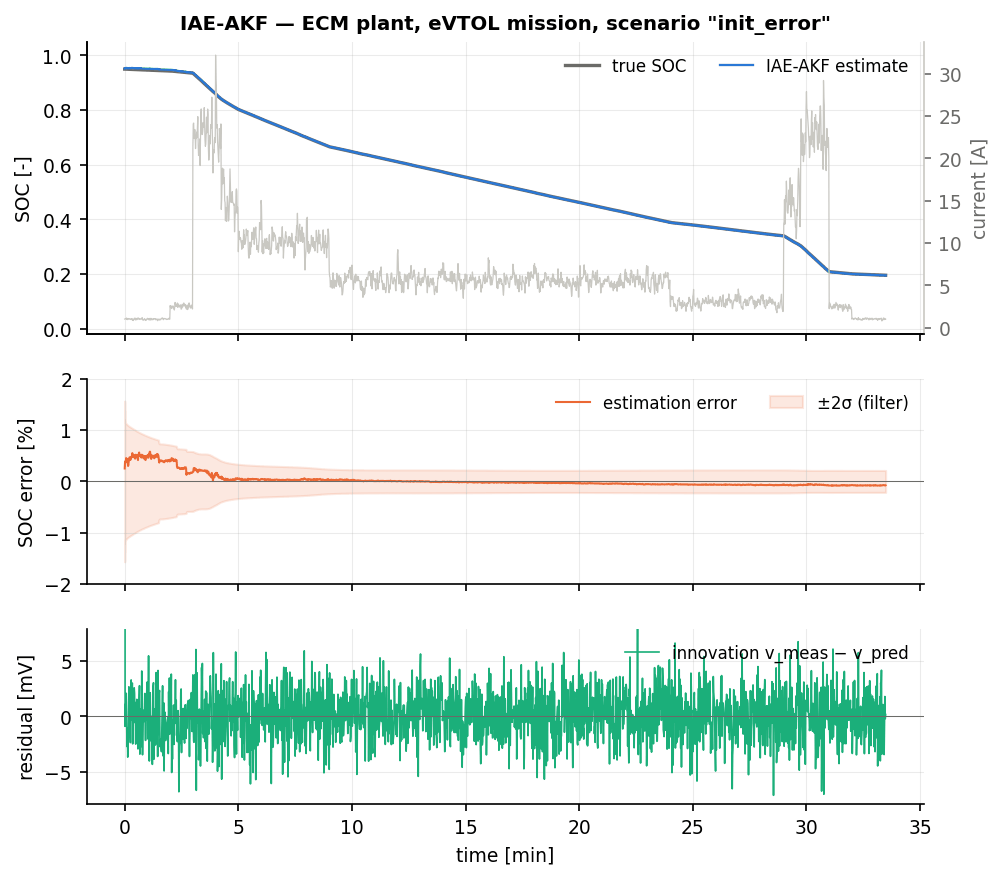
\includegraphics[width=\textwidth]{figures/cell_IAEAKF_init_error.png}
\caption{IAE-AKF with a 35\,\% initial SOC error.}
\end{figure}
\begin{figure}[H]\centering
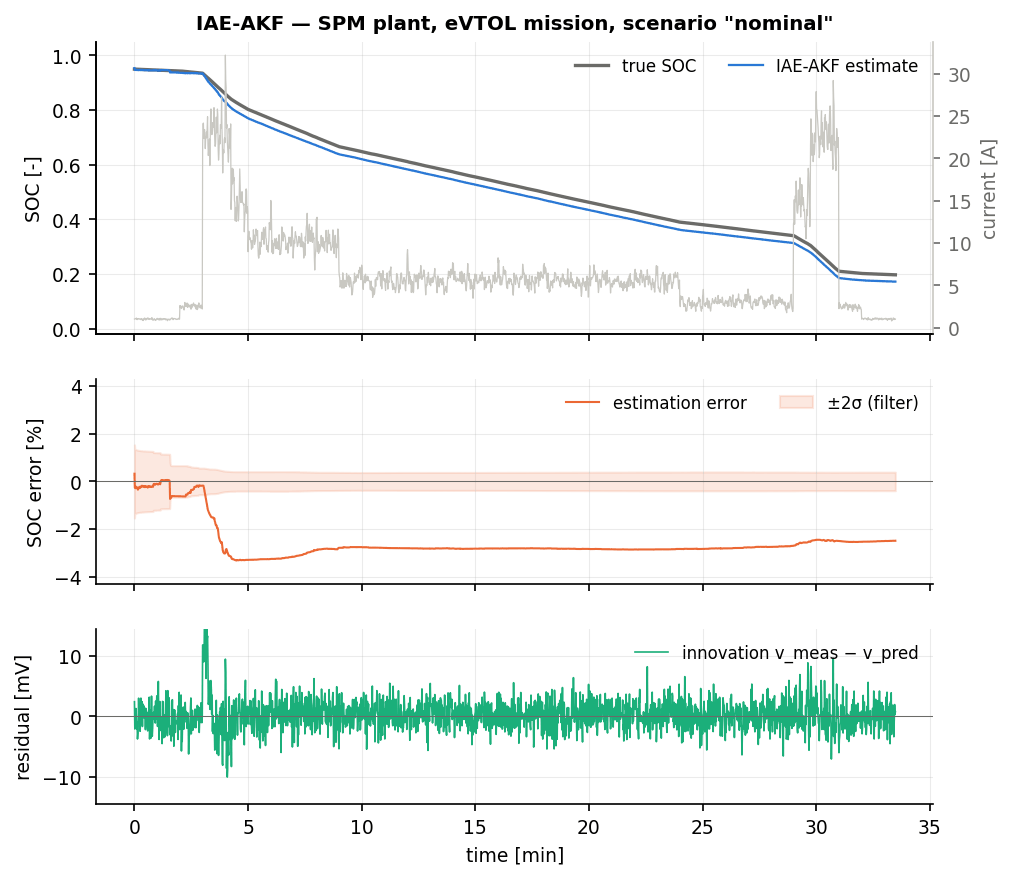
\includegraphics[width=\textwidth]{figures/cellspm_IAEAKF_nominal.png}
\caption{IAE-AKF on the electrochemical (single-particle) plant, nominal mission: the estimator uses a 2-RC ECM fitted to that plant and therefore sees a structured \SI{4}{\milli\volt} residual instead of white noise.}
\end{figure}

All figures below are three-seed means in \% SOC, as tabulated above; the plain \texttt{EKF} run on
the same data is the reference (\texttt{EKF ref.} column).  For orientation, the EKF scores
$\mathrm{rmse}_{ss}$ = 0.05\,\% on \texttt{nominal}, 0.12\,\% on \texttt{noise\_step}, 0.21\,\% on
\texttt{outliers}, 0.46\,\% on \texttt{sensor\_dropout}, 1.36\,\% on \texttt{param\_mismatch},
1.52\,\% on \texttt{aged\_cell} and 12.44\,\% on \texttt{combined} (where it never converges), and
3.73\,\% on the nominal SPM mission.

\paragraph{Benign scenarios.}  \texttt{nominal}: $\mathrm{rmse}=0.22\,\%$,
$\mathrm{rmse}_{ss}=\mathbf{0.04\,\%}$ against the EKF's $0.15\,\%$ / $0.05\,\%$.  The adaptation is
inactive in the useful sense --- $\hat\sigma_v$ hovers at \SI{2.15}{\milli\volt} against the nominal
\SI{2.13}{\milli\volt} --- and the filter is a plain EKF.  \texttt{init\_error}: converges at
$t=\SI{0}{\second}$ with $\mathrm{rmse}=0.12\,\%$ and $\mathrm{rmse}_{ss}=0.07\,\%$ (EKF $0.14\,\%$ /
$0.05\,\%$); the slightly larger steady-state value comes from the first $N$ samples, during which the
window fills with the very large innovations of the initial transient and $\hat{\mR}$ is briefly
inflated.  Both are far inside the $2\,\%$ acceptance bound.

\paragraph{Target scenario \texttt{noise\_step}.}  The estimated voltage-noise standard deviation
(seed 1) averages \SI{2.15}{\milli\volt} over $t\in[100,600)\,\si{\second}$ and
\SI{19.94}{\milli\volt} over $t\in[700,2010]\,\si{\second}$ --- within $0.3\,\%$ of the true
\SI{2}{\milli\volt}\,$\to$\,\SI{20}{\milli\volt} step once the \SI{0.6}{\milli\volt} contribution of
the current-sensor noise through $R_0$ is accounted for.  The SOC benefit is now unambiguous: the
EKF's steady-state error rises from $0.05\,\%$ on \texttt{nominal} to $0.12\,\%$ here because its
gain is a factor $\sqrt{92}$ too large for the new noise level, whereas IAE returns to
$\mathbf{0.04\,\%}$ --- a $3.0\times$ reduction, and the joint best of this family together with
Sage--Husa.  Consistency is restored exactly: the mean normalised innovation squared is $1.000$ both
before and after the step, against $1.099$ and $\mathbf{90.3}$ for the EKF.  The voltage-prediction
error falls from \SI{2.89}{\milli\volt} to \SI{1.01}{\milli\volt}, the best of all eight estimators in
this family.

\paragraph{Fault de-weighting.}  The clearest SOC benefit is on \texttt{sensor\_dropout}, where the
voltage reading is frozen at its value at $t=\SI{200}{\second}$ for \SI{15}{\second}.  The window
estimate reacts inside the fault: $\hat\sigma_v$ averages \SI{2.14}{\milli\volt} over
$[100,200)\,\si{\second}$, \SI{18.9}{\milli\volt} \emph{during} $[200,215)\,\si{\second}$ and
\SI{2.71}{\milli\volt} over $[215,400)\,\si{\second}$ --- an automatic, un-tuned nine-fold
de-weighting of a stuck sensor followed by a clean recovery.  The resulting metrics are
$\mathrm{rmse}=0.20\,\%$ and $\mathrm{rmse}_{ss}=\mathbf{0.05\,\%}$ against the EKF's $0.72\,\%$ and
$0.46\,\%$, improvements of $3.6\times$ and $9.2\times$ and the joint best of the whole family on this
scenario.  On \texttt{outliers} (5\,\% of samples corrupted by $\pm\SI{50}{\milli\volt}$) the filter
settles at $\hat\sigma_v=\SI{11.1}{\milli\volt}$ --- exactly the standard deviation of the
contaminated distribution --- and improves $\mathrm{rmse}$ from $0.52\,\%$ to $0.41\,\%$ and
$\mathrm{rmse}_{ss}$ from $0.21\,\%$ to $0.11\,\%$.  That is a real but modest gain: a uniformly
inflated $\mR$ is a blunt instrument against impulsive noise, and the variational filter of
\cref{ch:vbakf}, which reweights \emph{within} the sample, reaches $0.05\,\%$.

\paragraph{Model mismatch.}  \texttt{param\_mismatch}: $\mathrm{rmse}$ $1.28\to0.85\,\%$,
$\mathrm{rmse}_{ss}$ $1.36\to1.01\,\%$.  \texttt{aged\_cell}: $1.18\to1.06\,\%$,
$1.52\to1.21\,\%$.  \texttt{combined}: the EKF never reaches the $2\,\%$ band
($t_\mathrm{conv}=$ --, $16.02\,\%$ / $12.44\,\%$); the IAE filter converges at
$t=\SI{1448}{\second}$ with $4.89\,\%$ / $\mathbf{2.01\,\%}$, a $3.3\times$ / $6.2\times$
improvement.  The mechanism is the one analysed in \cref{ch:sagehusaakf}: the grown series
resistance puts a \SI{16}{\milli\volt} bias on the predicted voltage, the covariance-matching
estimator reads that bias as measurement noise, and the resulting de-weighting of the voltage channel
is the right thing to do for SOC because coulomb counting is the more trustworthy source on that
scenario.  The price is the voltage prediction, $\mathrm{rmse}_v$ rising from \SI{5.15}{\milli\volt}
to \SI{16.50}{\milli\volt} on \texttt{combined} and from \SI{3.80}{\milli\volt} to
\SI{24.50}{\milli\volt} on \texttt{aged\_cell} --- the largest voltage-prediction penalty in the
family, a direct consequence of the rectangular window's willingness to push $\hat{\mR}$ to its
ceiling.  \texttt{preisach} (Preisach hysteresis in the truth plant, corrected sign convention):
$0.61\,\%$ / $0.20\,\%$ against the EKF's $0.58\,\%$ / $0.20\,\%$ --- a draw in steady state, with
immediate convergence against the EKF's \SI{16}{\second}.  \texttt{cold} is also a draw
($0.16\,\%$ for both) and \texttt{current\_bias} is unchanged ($0.62\,\%$ against $0.61\,\%$), as it
must be: an input-side error does not inflate the innovations.

\paragraph{Comparison with Sage--Husa.}  The two estimators are within a few percent of each other on
almost every scenario, as the theory predicts --- they are the same covariance-matching idea with a
rectangular versus an exponential window.  IAE is faster (\SI{500}{\nano\second} against
\SI{545}{\nano\second}/step, both against the EKF's \SI{478}{\nano\second}), reacts to a fault
\emph{during} the fault rather than after it (because it adapts before the gain is formed), and is
better on \texttt{sensor\_dropout} ($0.05\,\%$ against $0.08\,\%$); Sage--Husa needs no buffer, is
structurally positive definite, and is better on \texttt{param\_mismatch} ($0.76\,\%$ against
$1.01\,\%$) and \texttt{outliers} ($0.06\,\%$ against $0.11\,\%$).

\paragraph{Electrochemical (SPM) plant.}  On the single-particle plant the estimator runs a 2-RC ECM
fitted to an electrochemical model with Butler--Volmer kinetics and a solid-diffusion time constant
of \SI{556}{\second}; the residual is therefore not white noise but a structured, slowly varying
\SI{4}{\milli\volt} signal.  IAE reaches $\mathrm{rmse}_{ss}=3.02\,\%$ on the nominal SPM mission
against the EKF's $3.73\,\%$ --- an $19\,\%$ improvement, and the best of the four $\mR$-adapting
filters, but far behind the covariance-inflating ones (Fading-EKF $0.36\,\%$, STF $0.66\,\%$).
Equation \eqref{eq:iae:R} is doing exactly what it was built to do and that is the problem: it
measures $\hat{\mC}_v\approx(\SI{4}{\milli\volt})^2$, subtracts the negligible
$\mH\Pminus\mH^\T$, concludes that the voltage channel carries four millivolts of noise, and lowers
the gain.  A lower gain means the SOC estimate is produced almost entirely by the coulomb integrator
--- and on the SPM plant the integrator is the faulty component, because the fitted capacity and
efficiency do not reproduce the true lithium inventory.  The voltage, by contrast, is informative:
the ECM's $\ocv(\soc)$ map was fitted to this plant, so inverting it would locate SOC to a few tenths
of a percent.  Under \emph{structured} model error the useful response is to shorten the filter's
memory so that recent measurements dominate the accumulated model (inflate $\mP$); covariance
matching does the opposite.  Where the SPM scenario piles a further error on top, the adaptation
helps as designed: \texttt{cold} $7.35\to2.54\,\%$ ($2.9\times$) and \texttt{param\_mismatch}
$3.13\to1.20\,\%$ ($2.6\times$).  SPM \texttt{outliers} is the one regression ($2.58\,\%$ against
$1.99\,\%$).

\section{Summary}
IAE is the most direct expression of covariance matching: measure the innovation covariance, subtract
what the filter already accounts for, and call the rest measurement noise.  Use it when the
measurement-noise level is uncertain or intermittently faulty and a fixed-length reaction time is
wanted --- here it tracks a tenfold noise step to within $0.3\,\%$ and cuts the SOC RMSE on a
stuck-sensor fault by a factor of nine and the error on a tenfold noise step from $0.12\,\%$ to
$0.04\,\%$.  On the electrochemical plant, where the residual is structured rather than white, it
gains only $19\,\%$ on the EKF ($3.02\,\%$ against $3.73\,\%$) while a fading-memory filter reaches
$0.36\,\%$ --- covariance matching lowers the gain, and under model error the useful move is the
opposite.  Do not use it when the innovations are strongly coloured
(it will over-estimate $\mR$), when the disturbance is impulsive rather than Gaussian (use a robust
update), or when you need to know \emph{why} the innovations grew --- covariance matching cannot
separate a noisy sensor from a wrong model.
